\documentclass{article}
\usepackage{geometry}
\usepackage{graphicx} % For including images
\usepackage{fancyhdr} % For customizing page header
\usepackage{eso-pic} % For setting background images
\usepackage{titlesec} % For customizing section headings

% Define page margins
\geometry{left=2.5cm,right=2.5cm,top=2.5cm,bottom=2.5cm}

\pagestyle{fancy}
\fancyhf{}
\renewcommand{\headrulewidth}{0pt} % Remove header rule line

% Add a logo or image to the header
\rhead{
\includegraphics[height=1.5cm]{pictures/lucky_logo.png}} 
\title{Company Information Report: Lucky Cement Limited}

\author{Zeeshan Zafar}
\date{\today}

% Define custom section formatting
\titleformat{\section}
{\normalfont\Large\bfseries\color{blue}} % Blue color for section headings
{}{0pt}{}

\begin{document}

\maketitle


% Create a minipage for the image on the left
\begin{minipage}[b]{0.5\textwidth}
  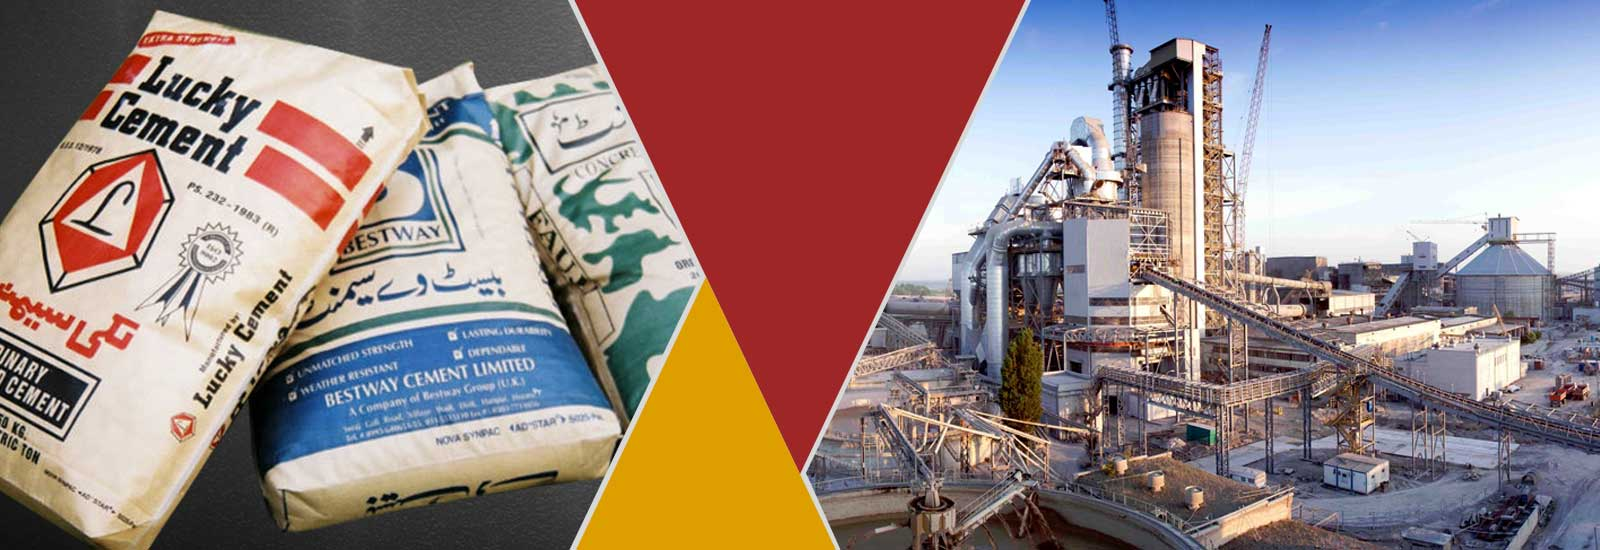
\includegraphics[width=1.5\textwidth, height=6cm, angle=90]{pictures/first.jpg}
\end{minipage}%
% Create a minipage for the introduction on the right (beside the image)
\begin{minipage}[b]{0.3\textwidth}
\vspace{40pt}

\section{Introduction}

  This report provides an insightful overview of Lucky Cement Limited, one of the leading companies in the cement manufacturing industry. Established on September 18, 1993, Lucky Cement Limited has played a pivotal role in the development of the construction and infrastructure sectors in Pakistan.

\vspace{12pt}
  The report covers key details such as the company's incorporation name, registered office location, incorporation date, and the type of liability structure it operates under. Furthermore, it includes information about the company's share capital, the total number of shares, and their cost per share.

\vspace{12pt}
  This report serves as a valuable resource for stakeholders, investors, and anyone interested in gaining insights into Lucky Cement Limited's operations, history, and contributions to the cement industry in Pakistan.
\end{minipage}

\newpage


\vspace{42pt}
\section{Company Details}
\vspace{22pt}
\subsection{Incorporation Name}
The incorporation name of the company is \textbf{Lucky Cement Limited}.

\vspace{22pt}
\subsection{Registered Office}
The registered office of Lucky Cement Limited is located at:
\begin{quote}
6-A, Muhammad Ali Housing Society, \\
A. Aziz Hashim Tabba Street, \\
Karachi-75350, \\
Pakistan
\end{quote}

\vspace{22pt}
\subsection{Incorporation Date}
Lucky Cement Limited was incorporated on \textbf{September 18, 1993}.

\vspace{22pt}
\subsection{Type of Liability}
Lucky Cement Limited is associated with \textbf{limited liability}. Shareholders have limited liability, and their personal assets are protected beyond their shareholdings.

\begin{figure}[b]
  \centering
  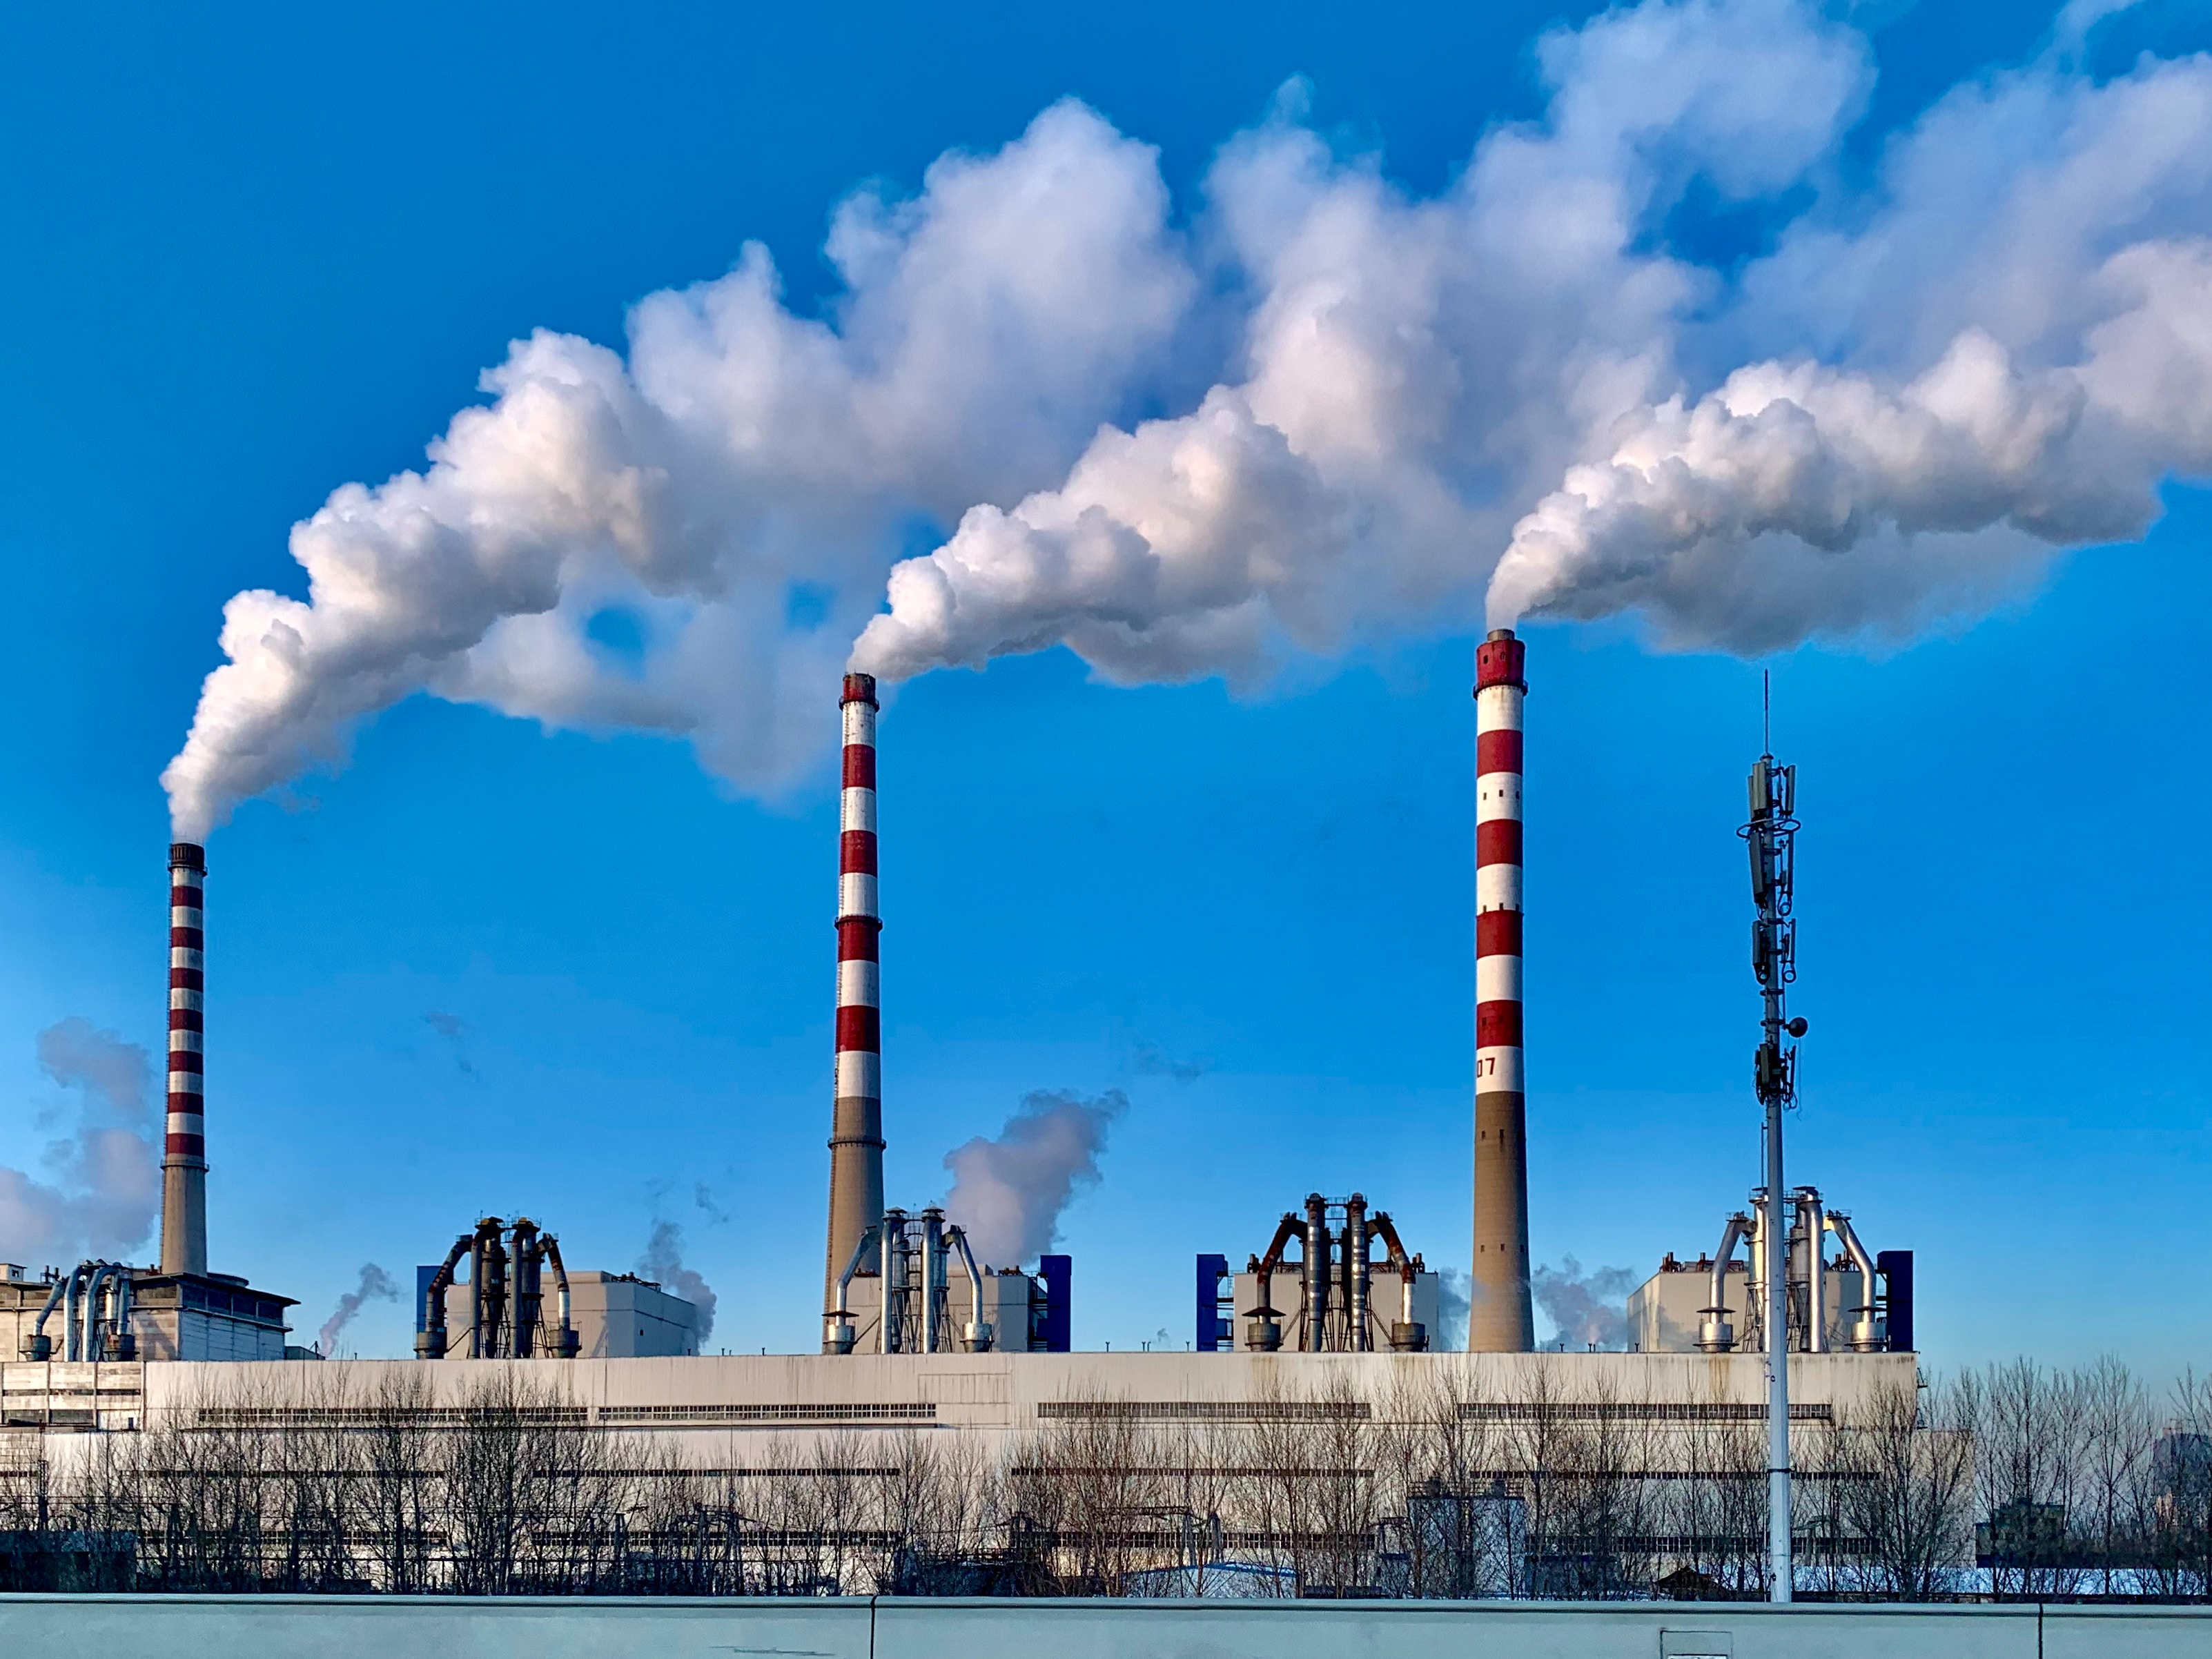
\includegraphics[width=1.1\textwidth, height=6.5cm]{pictures/second.jpg}
\end{figure}

\newpage






% Set the background image for the next page (Share Capital section)
\AddToShipoutPictureBG*{%
  \AtPageLowerLeft{%
    
\includegraphics[width=\paperwidth, height=\paperheight]{pictures/third.jpg} % Specify the background image file
  }%
}



% Section with background image
\section{Share Capital}

\vspace{22pt}
% Create a minipage for the content in the Share Capital section
\begin{minipage}[b]{0.6\textwidth}
  \subsection{Starting Share Capital}
  The starting share capital of Lucky Core Industry Karachi was  \textbf{PKR 1 billion}. The total number of shares was  \textbf{100 million}, and the cost per share was  \textbf{PKR 10}.
  
  \subsection{Current Share Capital}
  The current share capital of Lucky Core Industry Karachi is  \textbf{PKR 15 billion}. The total number of shares is  \textbf{1.5 billion}, and the cost per share is  \textbf{PKR 10}.
  
  The company has increased its share capital over time through a number of right issues. The most recent right issue was in  \textbf{2022}, when the company raised  \textbf{PKR 5 billion}.

 \vspace{15pt}
   \textbf{Note:} The cost per share is the price at which the shares are traded on the stock exchange. It can fluctuate depending on market conditions.
\end{minipage}

% Remove the background image after this page
\ClearShipoutPictureBG






\newpage

% Set text color to white for this page
\color{white}

% Set the background image for the next page (Share Capital section)
\AddToShipoutPictureBG*{%
  \AtPageLowerLeft{%
    
\includegraphics[width=\paperwidth, height=\paperheight]{pictures/fourth.jpg} % Specify the background image file
  }%
}

\section{Terms for the Working of Directors}

 \vspace{22pt}
The terms defined for the working of the directors of Lucky Cement Limited (LCI) are as follows:

 \vspace{22pt}
\begin{enumerate}
  \item \textbf{Appointment:} Directors are appointed by the shareholders at the annual general meeting.
  \item \textbf{Tenure:} Directors hold office for a period of three years, but are eligible for re-election at the end of their term.
  \item \textbf{Remuneration:} Directors are paid a remuneration for their services, which is determined by the board of directors.
  \item \textbf{Duties and Responsibilities:} The directors are responsible for the overall management and control of the company. They are also responsible for ensuring that the company complies with all applicable laws and regulations.
\end{enumerate}

 \vspace{22pt}
In addition to the above terms, the directors of LCI are also subject to the following specific provisions:

 \vspace{22pt}
\begin{itemize}
  \item \textbf{Code of Conduct:} The directors are required to comply with the company's Code of Conduct, which sets out ethical standards and guidelines for their behavior.
  \item \textbf{Conflict of Interest:} The directors are required to disclose any conflicts of interest to the board of directors.
  \item \textbf{Indemnification:} The company indemnifies the directors against certain liabilities incurred in the course of their duties.
\end{itemize}

% Remove the background image after this page
\ClearShipoutPictureBG



\newpage
% Set text color to white for this page
\color{black}
\section{Conclusion}
 \vspace{22pt}
This report provides key information about Lucky Cement Limited, including its  \textbf{incorporation name},  \textbf{registered office},  \textbf{incorporation date},  \textbf{type of liability}, \textbf{share capital,directors} etc. Overall 
 \textbf{Lucky Cement Limited (LCI)} is a leading cement producer and exporter in Pakistan with a  \textbf{strong} track record and a  \textbf{bright} future. The company is well-positioned to benefit from the continued  \textbf{growth} of the construction industry in Pakistan and other  \textbf{markets} in the region.
\end{document}
